\section{Inequality constraints in QAOA: QOBLIB portfolio optimisation}\label{sec:portfolio}
This appendix uses the constraint automaton to encode \emph{inequality} constraints in QAOA~\cite{farhi2014,hadfield2019}, on class \texttt{06-portfolio} of the Quantum Optimization Benchmarking Library (QOBLIB)~\cite{koch2026qoblib}.

\paragraph{Model.} At each period $t$ the investor holds long and short positions $x_{t,d,i}\in\{0,1\}$ ($d\in\{\mathrm{long},\mathrm{short}\}$, one unit per asset, \texttt{ub}$=1$). The objective (risk, return, transaction, short-selling and liquidation costs, cash interest) is the reference model \texttt{bqp\_u3\_c10}; our implementation reproduces the official QOBLIB checker exactly, including the reference value $-1595$ of the ISQR submission for \texttt{po\_a003\_t02\_orig}. Each period has two inequalities, $0\le C-(L_t-S_t)\le 2^{c_1}-1$ (capital) and $0\le B-(L_t+S_t)\le 2^{c_2}-1$ (budget), where $L_t,S_t$ count long and short positions. We use $C=3$, $B=3$ or $4$, and the risk weights of the ISQR submission ($10^{-5}$--$4\cdot10^{-5}$) or a QOBLIB \texttt{l1e-5} variant. This is a derived model, not the QOBLIB reference variant (three units, $C=10$), so optimal values are not comparable with the QOBLIB table. Exact optima and worst feasible values come from a dynamic programme over periods.

\paragraph{Encodings compared.} (i) The official QUBO, with $T(c_1+c_2)$ binary slack qubits and a quadratic penalty. (ii) Unbalanced penalisation~\cite{montanez2024unbalanced}, which needs no slack qubits. (iii) The negation-forced state $A_q|0\rangle$ as initial state: a variable is forced when its other value would make the period's constraints impossible to complete (exact look-ahead on the counters $(L,S)$), so the support is exactly the feasible set and there are no dead ends. It is combined with the X mixer, with an XY mixer~\cite{wang2020xy} inside each (period, direction) block, which conserves $L_t$ and $S_t$ and hence feasibility, or with the Grover mixer about $A_q|0\rangle$~\cite{bartschi2020gm} (CG-QAOA). With (iii) the phase operator contains only the objective, without any penalty term. \Cref{fig:hybrid} shows the hybrid circuit.

\begin{figure*}[t]\centering
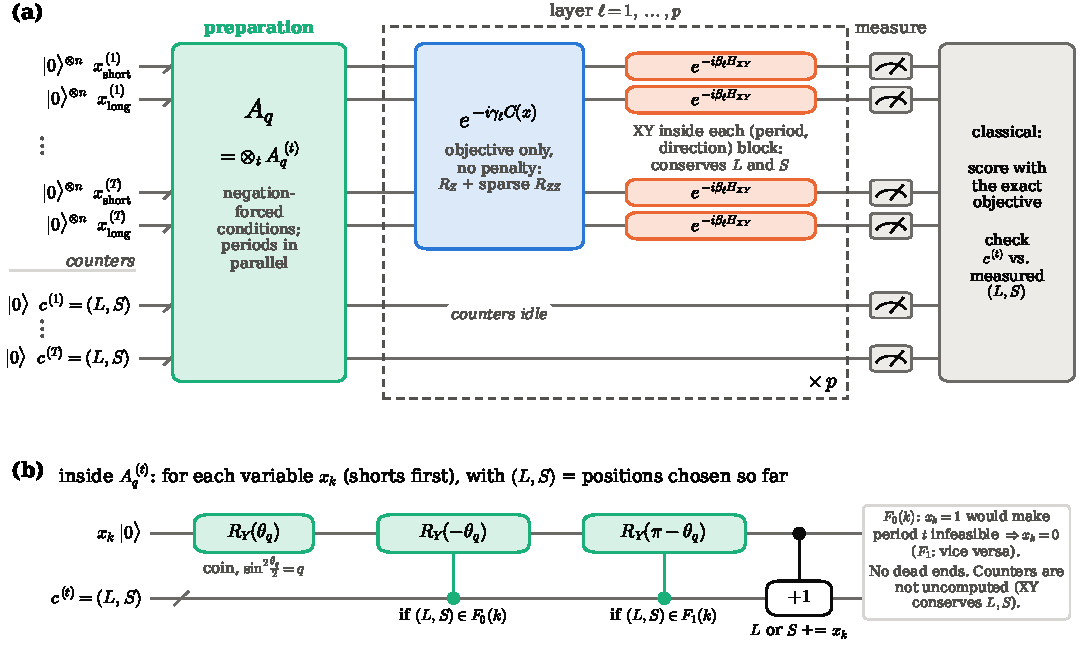
\includegraphics[width=\textwidth]{figures/fig_hybrid_blocks.pdf}
\caption{Hybrid constraint-guided QAOA. (a) Inequalities are enforced once by $A_q=\bigotimes_t A_q^{(t)}$ (periods in parallel); each layer applies the objective-only phase and an XY mixer inside each (period, direction) block, which conserves $(L,S)$. (b) One variable inside $A_q^{(t)}$: coin $R_Y(\theta_q)$, counter-controlled correction when $x_k$ is forced to 0 ($F_0$) or 1 ($F_1$), counter increment. Counters need no uncomputation because XY conserves the counts.}\label{fig:hybrid}
\end{figure*}

\paragraph{Exact simulation.} \Cref{tab:pf_exact,fig:pf_quality} report $p=1,2,3$ on three QOBLIB instances (12, 16, 20 decision qubits). Penalty weights are tuned over $\alpha\in[1/64,8]$ times the largest linear coefficient, and the best value is kept. Five observations: (1)~$A_q$ followed by the X mixer leaks out of the feasible set and ends below $A_q$ alone at every depth: \emph{the constraint-guided state helps only with a constraint-preserving mixer}. (2)~The hybrid ($A_q$ + XY) is 100\,\% feasible and has higher quality and higher P(optimum) than both penalty encodings at every depth on every instance. (3)~CG-QAOA is best in quality and P(optimum). (4)~If infeasible samples are discarded classically, the surviving penalty samples are as good as or better than the hybrid's on the two smaller instances: the hybrid's gain on these two instances is only that it does not waste shots on infeasible samples. (5)~$A_q$ alone is classically samplable and already strong; the QAOA layers add up to $13\times$ in P(optimum) on top of it.

\begin{figure*}[t]\centering
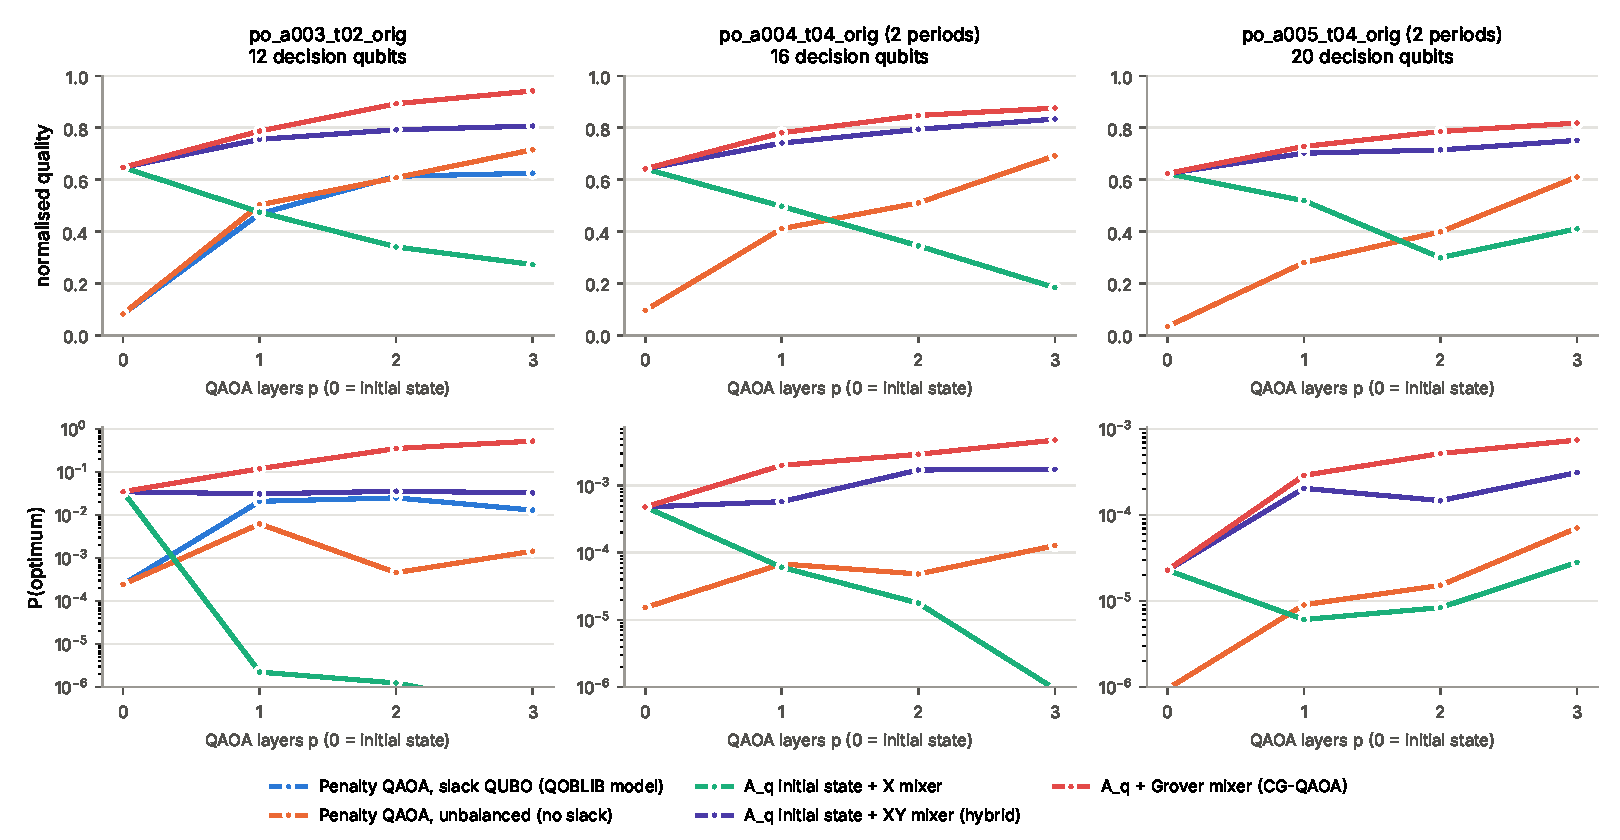
\includegraphics[width=0.92\textwidth]{figures/fig_portfolio_quality.pdf}
\caption{\orig{exact ideal simulation} Exact simulation, QOBLIB portfolio instances: normalised quality (infeasible = 0) and P(optimum) vs.\ QAOA depth. $p=0$ is the initial state.}\label{fig:pf_quality}
\end{figure*}
\begin{table*}[t]\centering\small
\caption{\orig{exact ideal simulation} Exact simulation on QOBLIB portfolio instances: P(feasible) / normalised quality (infeasible samples count 0) / P(optimum) for $p=1,2,3$. Penalty weights tuned over $\alpha\in[1/64,8]$; best value kept. $p=0$: uniform sampling (penalty rows) or $A_q$ alone (classically samplable).}\label{tab:pf_exact}
\resizebox{\linewidth}{!}{\begin{tabular}{llcccc}\toprule instance (qubits ours/slack) & method & $p=0$ & $p=1$ & $p=2$ & $p=3$\\\midrule
\texttt{a003\_t02} (12/20) & Penalty, slack QUBO & 0.17 / 0.08 / 2.4e-4 & 0.58 / 0.47 / 2.1e-2 & 0.72 / 0.61 / 2.5e-2 & 0.77 / 0.62 / 1.3e-2\\
 & Penalty, unbalanced & 0.17 / 0.08 / 2.4e-4 & 0.63 / 0.50 / 6.2e-3 & 0.79 / 0.61 / 4.6e-4 & 0.81 / 0.72 / 1.4e-3\\
 & $A_q$ + X mixer & 1.00 / 0.65 / 3.5e-2 & 0.96 / 0.47 / 2.2e-6 & 0.70 / 0.34 / 1.2e-6 & 0.57 / 0.27 / 3.0e-7\\
 & $A_q$ + XY (hybrid) & 1.00 / 0.65 / 3.5e-2 & 1.00 / 0.76 / 3.1e-2 & 1.00 / 0.79 / 3.6e-2 & 1.00 / 0.81 / 3.3e-2\\
 & $A_q$ + Grover (CG-QAOA) & 1.00 / 0.65 / 3.5e-2 & 1.00 / 0.79 / 1.2e-1 & 1.00 / 0.89 / 3.5e-1 & 1.00 / 0.94 / 5.3e-1\\
\midrule
\texttt{a004\_t04} (2 per.) (16/26) & Penalty, unbalanced & 0.17 / 0.10 / 1.5e-5 & 0.56 / 0.41 / 6.8e-5 & 0.61 / 0.51 / 4.8e-5 & 0.81 / 0.69 / 1.3e-4\\
 & $A_q$ + X mixer & 1.00 / 0.64 / 4.8e-4 & 0.81 / 0.50 / 6.1e-5 & 0.55 / 0.34 / 1.8e-5 & 0.29 / 0.18 / 9.4e-7\\
 & $A_q$ + XY (hybrid) & 1.00 / 0.64 / 4.8e-4 & 1.00 / 0.74 / 5.8e-4 & 1.00 / 0.79 / 1.7e-3 & 1.00 / 0.83 / 1.7e-3\\
 & $A_q$ + Grover (CG-QAOA) & 1.00 / 0.64 / 4.8e-4 & 1.00 / 0.78 / 2.0e-3 & 1.00 / 0.85 / 2.9e-3 & 1.00 / 0.88 / 4.8e-3\\
\midrule
\texttt{a005\_t04} (2 per.) (20/30) & Penalty, unbalanced & 0.06 / 0.03 / 9.5e-7 & 0.43 / 0.28 / 9.0e-6 & 0.55 / 0.40 / 1.5e-5 & 0.84 / 0.61 / 7.1e-5\\
 & $A_q$ + X mixer & 1.00 / 0.62 / 2.3e-5 & 0.87 / 0.52 / 6.1e-6 & 0.48 / 0.30 / 8.4e-6 & 0.68 / 0.41 / 2.8e-5\\
 & $A_q$ + XY (hybrid) & 1.00 / 0.62 / 2.3e-5 & 1.00 / 0.70 / 2.0e-4 & 1.00 / 0.71 / 1.5e-4 & 1.00 / 0.75 / 3.1e-4\\
 & $A_q$ + Grover (CG-QAOA) & 1.00 / 0.62 / 2.3e-5 & 1.00 / 0.73 / 2.9e-4 & 1.00 / 0.79 / 5.2e-4 & 1.00 / 0.82 / 7.4e-4\\
\bottomrule\end{tabular}}\end{table*}


\paragraph{Reducing depth.} \Cref{tab:pf_depth} follows the hybrid through four versions on \texttt{ibm\_fez}. v1 (counters uncomputed) costs 511--1857 CZ at $p=1$ and the Grover mixer 4\,000--13\,000 CZ per layer, beyond current devices. v2 orders the shorts first, which leaves fewer forced counter states, and keeps one counter pair per period without uncomputation; the counters then hold $(L_t,S_t)$, which XY conserves, so all statistics on $x$ are unchanged (verified against the exact state). This halves $A_q$ (324$\to$150 CZ on 12 qubits). v3 drops the small risk couplings from the phase and uses XY on a path. Constraints sit in the state, not in the cost, so this does not lower the ideal quality, whereas a penalty is quadratic by construction. Together v1$\to$v3 removes 65--75\,\% of the CZ gates and 75--82\,\% of the depth. Off-the-shelf ZX simplification did not help here: PyZX \texttt{full\_reduce} with extraction roughly doubles the CZ count and phase teleportation is neutral (within 8\,\%). Comparing all-to-all with heavy-hex compilation shows that about 40\,\% of the remaining CZ gates are routing, which architecture-aware synthesis could target.

\paragraph{Classicality as a design tool.} Feasibility depends only on the counts $(L_t,S_t)$, because every unit has the same cash value, and neither XY nor the phase changes them. Different count sectors therefore never interfere, and the logic of the negative conditions can be executed classically, which is an instance of the idea behind the classicality lemma (\cref{sec:classical}). Draw $(L_t,S_t)$ per shot from the weights of $A_q$, either offline or with a mid-circuit-measured coin, and let the chip prepare only the superposition over \emph{which} assets, a Dicke state per block~\cite{bartschi2019dicke}, followed by the XY layers. Measuring the decision qubits themselves, by contrast, destroys the gain (quality $0.76\to0.64$). The same statistics are obtained coherently and without ancillas: a weighted ``thermometer'' state of the counts followed by the Dicke unitary $U_{n,k}$ of Ref.~\cite{bartschi2019dicke}, which we verified to coincide exactly with the per-shot construction. With counts drawn per shot the 12-qubit circuit needs 24 (40) CZ at $p=1$ ($p=2$) instead of 178 (200), with quality 0.74 (0.84).

\begin{table}[t]\centering\small
\caption{\orig{compiled counts} CZ gates / depth on \texttt{ibm\_fez} (FakeFez, level 3) for one and two layers. v1: counters uncomputed; v2: shorts-first order, lean counters; v3: v2 + path XY + linear phase; counts+Dicke: counts drawn classically, Dicke preparation (most expensive count sector).}\label{tab:pf_depth}
\resizebox{\linewidth}{!}{\begin{tabular}{lccc}\toprule circuit & a003 (12) & a004 (16) & a005 (20)\\\midrule
penalty, slack QUBO, $p=1$ & 311/312 & 588/460 & 854/664\\
penalty, unbalanced, $p=1$ & 92/128 & 185/184 & 301/279\\
hybrid v1, $p=1$ & 511/952 & 1323/2291 & 1857/3053\\
hybrid v2, $p=1$ & 330/387 & 762/696 & 1064/936\\
hybrid v3, $p=1$ & 178/225 & 446/567 & 541/652\\
counts+Dicke, $p=1$ & 24/32 & 156/127 & --\\
\midrule
penalty, slack QUBO, $p=2$ & 693/639 & 1231/986 & 1863/1219\\
penalty, unbalanced, $p=2$ & 206/258 & 408/422 & 674/610\\
hybrid v1, $p=2$ & 678/1361 & 1618/2982 & 2400/3456\\
hybrid v2, $p=2$ & 481/567 & 1100/1040 & 1617/1635\\
hybrid v3, $p=2$ & 200/255 & 454/528 & 601/690\\
counts+Dicke, $p=2$ & 40/49 & 184/148 & --\\
\midrule
CG-QAOA (Grover mixer), $p=1$ & 4013/9882 & 9203/20872 & 13364/31631\\
\bottomrule\end{tabular}}\end{table}


\paragraph{Noise.} \Cref{tab:pf_noise,fig:pf_noise} use the \texttt{ibm\_fez} noise model on \texttt{po\_a003\_t02\_orig}. Feasibility is no longer guaranteed, and the first hybrid (531 CZ) is worse than unbalanced penalty QAOA. The hardware-friendly versions reverse this: counts+Dicke reaches quality 0.70--0.75 with 27--52 CZ per shot, against at most 0.50 for any penalty circuit, and P(optimum) 4.5\,\% against at most 1\,\%.

\begin{table}[t]\centering\small
\caption{\orig{gate-level noisy simulation (FakeFez noise model); no hardware} \texttt{po\_a003\_t02\_orig} under the \texttt{ibm\_fez} noise model (FakeFez, 2000--4000 shots).}\label{tab:pf_noise}
\resizebox{\linewidth}{!}{\begin{tabular}{lcccc}\toprule circuit & CZ & P(feas.) & quality & P(opt)\\\midrule
penalty, unbalanced, $p=1$ & 101 & 0.60 & 0.47 & 0.8\%\\
penalty, slack, $p=1$ & 339 & 0.47 & 0.36 & 0.9\%\\
penalty, unbalanced, $p=2$ & 206 & 0.68 & 0.50 & 0.1\%\\
penalty, slack, $p=2$ & 693 & 0.52 & 0.39 & 1.0\%\\
$A_q$ alone (lean, classically samplable) & 150 & 0.92 & 0.59 & 2.1\%\\
hybrid v1, $p=1$ & 531 & 0.59 & 0.39 & 1.4\%\\
hybrid v3, $p=1$ & 178 & 0.85 & 0.63 & 2.4\%\\
hybrid v3, $p=2$ & 200 & 0.80 & 0.63 & 1.0\%\\
counts+Dicke, $p=1$ & 27 & 0.95 & 0.70 & 4.5\%\\
counts+Dicke, $p=2$ & 52 & 0.90 & 0.75 & 1.2\%\\
\bottomrule\end{tabular}}\end{table}

\begin{figure}[t]\centering
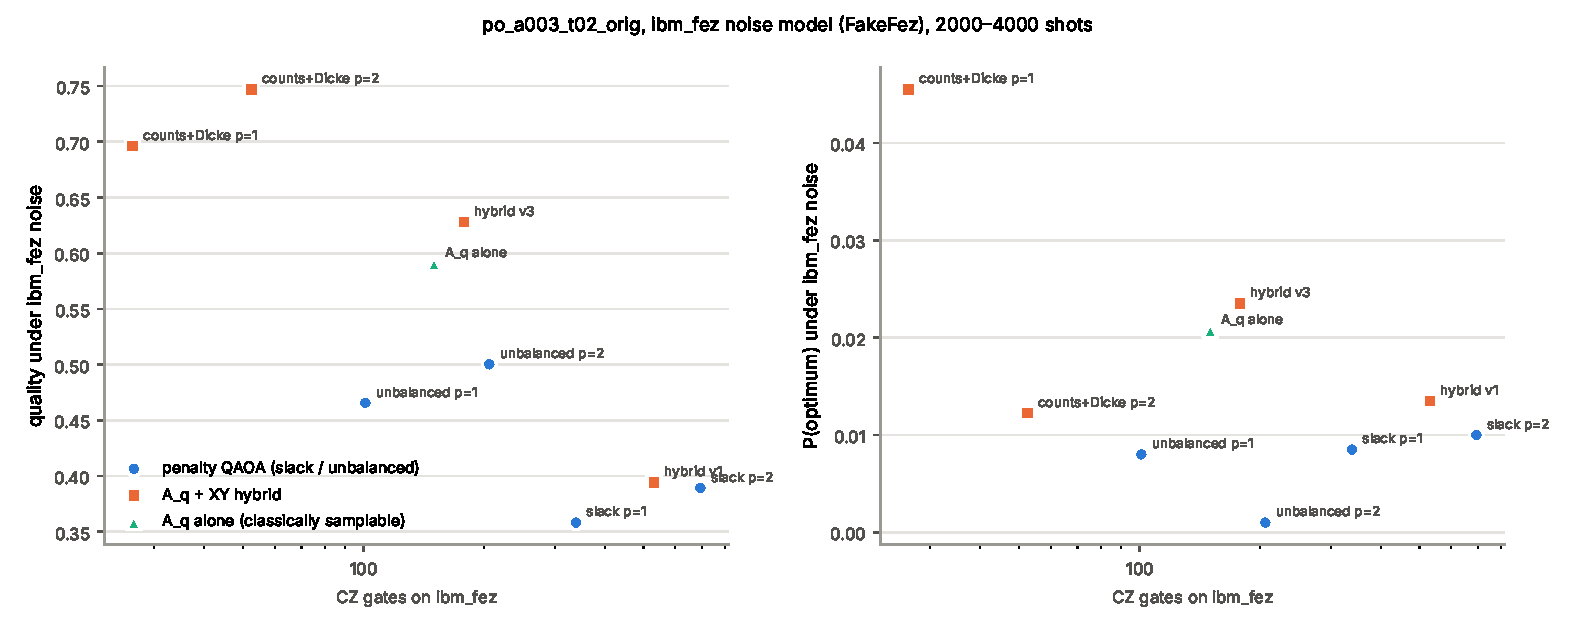
\includegraphics[width=\columnwidth]{figures/fig_portfolio_noisy.pdf}
\caption{\orig{gate-level noisy simulation; no hardware} Quality and P(optimum) vs.\ CZ count under the \texttt{ibm\_fez} noise model (\texttt{po\_a003\_t02\_orig}).}\label{fig:pf_noise}
\end{figure}

\paragraph{Scaling to 300 qubits.} \Cref{tab:pf_scaling,fig:pf_scaling} use Qiskit Aer's MPS simulator on seven QOBLIB instances, from 12 to 300 decision qubits (\texttt{a003\_t02} to \texttt{a010\_t15}), at $p=1$. Angles were transferred from the exactly optimised small instances (phase in units of the largest linear coefficient) and refined on a grid. Bond dimension 64 agrees with 256 and, on 12 qubits, with the exact statevector. The fair classical baseline draws the same counts and a uniform subset of assets. Unbalanced penalty QAOA falls from 64\,\% feasible samples to 0 of 2000 at 300 qubits; the hybrid stays at 100\,\%. It exceeds the classical baseline in quality by 0.04--0.15 at every size, and its best of 2000 shots is 1.2--4.8 times closer to the exact optimum. Where the circuits fit on \texttt{ibm\_fez}, the per-shot hybrid is the cheapest, and the single coherent circuit is cheaper than the penalty circuit from 80 qubits on.

\begin{figure*}[t]\centering
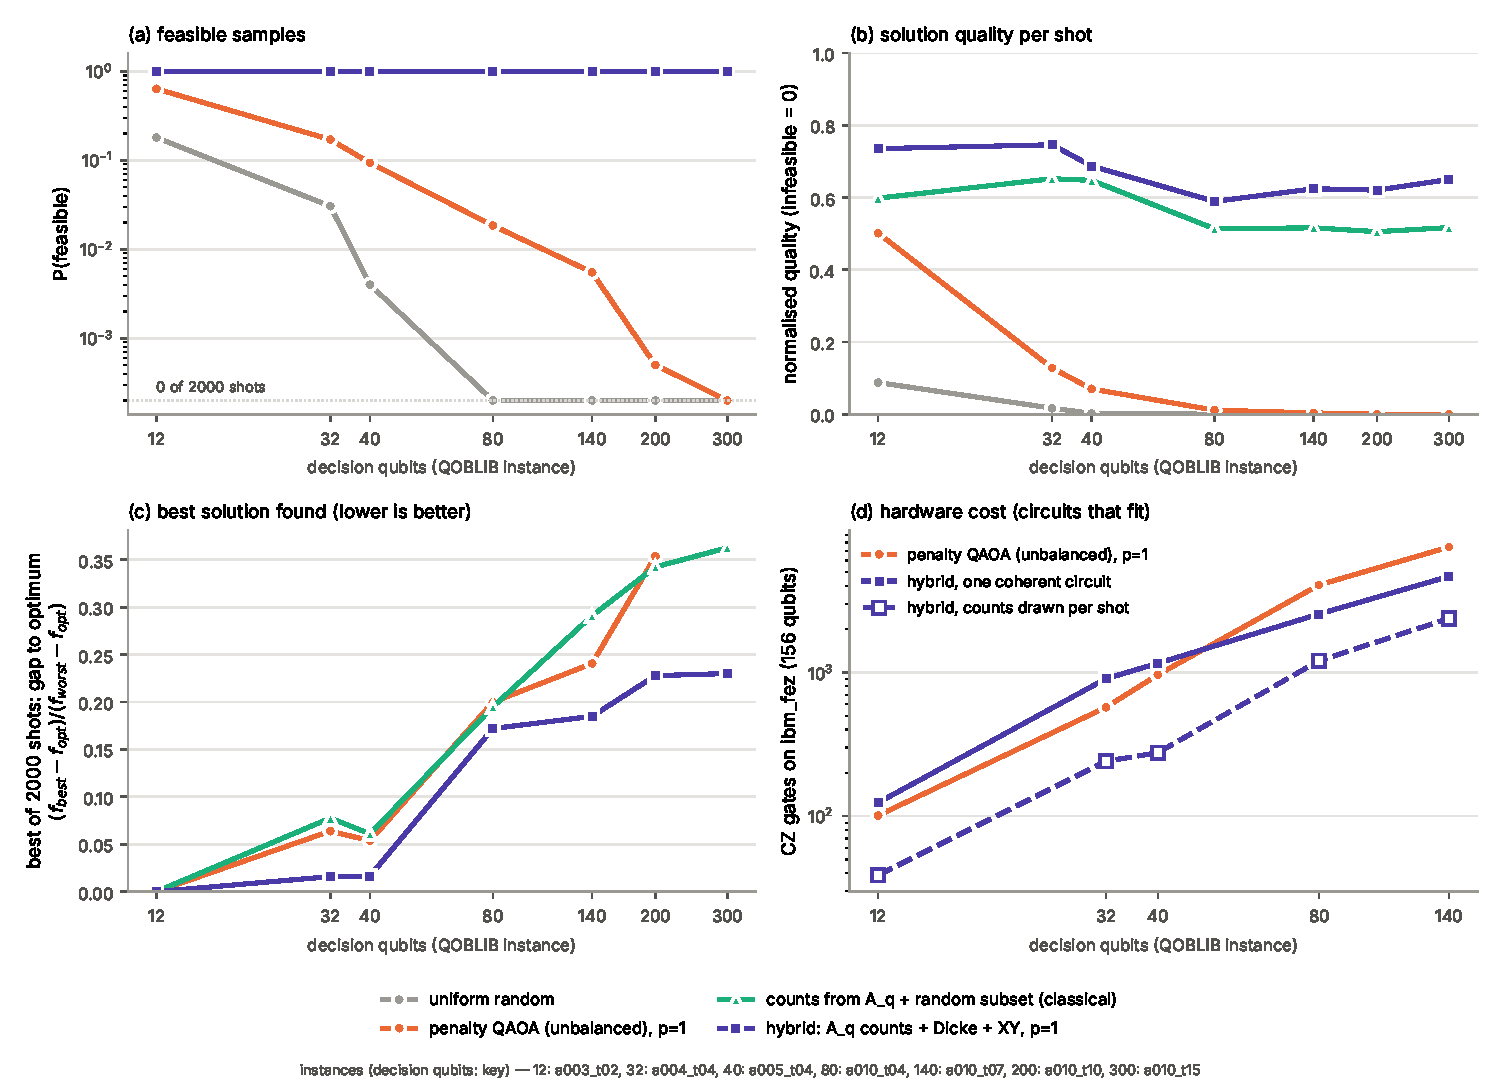
\includegraphics[width=0.9\textwidth]{figures/fig_portfolio_scaling.pdf}
\caption{\orig{ideal matrix-product-state simulation and compiled counts} QOBLIB portfolio instances from 12 to 300 decision qubits (Aer MPS, $p=1$, 2000 shots): feasibility, quality, best-shot gap to the exact optimum, and CZ count on \texttt{ibm\_fez}.}\label{fig:pf_scaling}
\end{figure*}
\begin{table*}[t]\centering\small
\caption{\orig{ideal matrix-product-state simulation and compiled counts} Aer MPS simulation (bond dimension 64), $p=1$, 2000 shots. Quality: normalised, infeasible = 0; gap: best of 2000 shots, $(f_{best}-f_{opt})/(f_{worst}-f_{opt})$, exact $f_{opt}$ by dynamic programming. CZ on \texttt{ibm\_fez} only where the circuit fits (156 qubits).}\label{tab:pf_scaling}
\resizebox{\linewidth}{!}{\begin{tabular}{lrrcccccccc}\toprule & & & \multicolumn{2}{c}{P(feasible)} & \multicolumn{3}{c}{quality} & \multicolumn{2}{c}{best-shot gap} & CZ (pen./hyb./per shot)\\
instance & qubits & slack QUBO & pen. & hyb. & pen. & classical & hyb. & classical & hyb. & \\\midrule
\texttt{a003\_t02} & 12 & 20 & 0.6355 & 1 & 0.501 & 0.598 & 0.735 & 0.000 & 0.000 & 101/124/39\\
\texttt{a004\_t04} & 32 & 52 & 0.1710 & 1 & 0.128 & 0.652 & 0.746 & 0.078 & 0.016 & 572/904/241\\
\texttt{a005\_t04} & 40 & 60 & 0.0935 & 1 & 0.070 & 0.648 & 0.687 & 0.061 & 0.016 & 963/1158/276\\
\texttt{a010\_t04} & 80 & 100 & 0.0185 & 1 & 0.011 & 0.514 & 0.589 & 0.195 & 0.172 & 4056/2546/1205\\
\texttt{a010\_t07} & 140 & 175 & 0.0055 & 1 & 0.004 & 0.516 & 0.625 & 0.291 & 0.185 & 7452/4655/2376\\
\texttt{a010\_t10} & 200 & 250 & 0.0005 & 1 & 0.000 & 0.505 & 0.621 & 0.342 & 0.228 & --\\
\texttt{a010\_t15} & 300 & 375 & 0.0000 & 1 & 0.000 & 0.517 & 0.650 & 0.363 & 0.230 & --\\
\bottomrule\end{tabular}}\end{table*}


\paragraph{Limitations of this study.} (i)~With a linear phase and XY on paths, entanglement stays inside blocks of $n$ qubits. That is why MPS scales, and it also means this regime is classically simulable: we claim a better \emph{encoding}, not a quantum advantage, and classical MIQP solvers solve all these instances~\cite{babbush2021}. (ii)~The counts trick needs constraints that depend only on counts. Weighted constraints (multiple knapsack) need the coherent $A_q$ with counters, or the indicator oracles of Ref.~\cite{bucher2025}. (iii)~Most of the gain comes from the count distribution, which is classical; the quantum layers add a consistent but moderate improvement. (iv)~The noise results are simulations of a noise model and cover one instance; no device run is reported. (v)~Angles at large sizes come from transfer plus a grid, not a full optimisation. (vi)~The model is a derived QOBLIB variant (\texttt{ub}$=1$).
